% 2009 年安徽卷文科第 17 题：待填写的茎叶图空白表。
% 来源 PDF：普通高考/2009/2009安徽文.pdf，SHA256 83b982d22fd84a0158f909bce3d1f62e1fa228868e7915ded21e7a5ed9774897
% 原页：第 1 页（A3 三栏）第 3 栏下部，印刷页 497。
% 重绘依据：表头左「A」右「B」，中间为茎（35–45），两侧留空供填写叶；按原图保留竖线与横线。
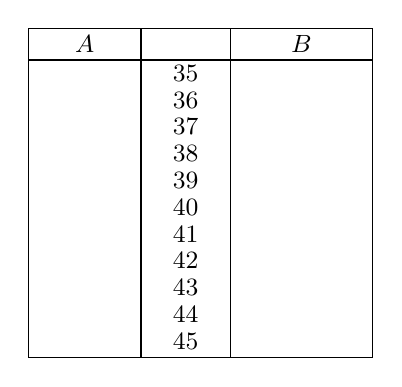
\begin{tikzpicture}[scale=0.95, semithick, every node/.style={inner sep=2.2pt, font=\small}]
  \draw (0,0) rectangle (4.6,-4.4);
  \draw (1.5,0) -- (1.5,-4.4);
  \draw (2.7,0) -- (2.7,-4.4);
  \draw (0,-0.42) -- (4.6,-0.42);
  \node at (0.75,-0.21) {$A$};
  \node at (3.65,-0.21) {$B$};
  \foreach \i/\s in {0/35,1/36,2/37,3/38,4/39,5/40,6/41,7/42,8/43,9/44,10/45} {
    \node at (2.1,{-0.42-(\i+0.5)*0.358}) {$\s$};
  }
\end{tikzpicture}
